\documentclass[10pt]{article}

% --- NeurIPS 2026 workshop format approximation ---
\usepackage[utf8]{inputenc}
\usepackage[T1]{fontenc}
\usepackage{times}
\usepackage[margin=1in]{geometry}
\usepackage{amsmath,amssymb,amsthm}
\usepackage{mathtools}
\usepackage{bm}
\usepackage{graphicx}
\usepackage{booktabs}
\usepackage{hyperref}
\usepackage{url}
\usepackage{microtype}
\usepackage{natbib}
\usepackage{xcolor}
\usepackage{enumitem}
\usepackage{caption}
\usepackage{subcaption}
\usepackage{wrapfig}
\usepackage{algorithm}
\usepackage{algorithmic}

% Attempt to load neurips_2026; fall back gracefully
\IfFileExists{neurips_2026.sty}{\usepackage{neurips_2026}}{}

% --- Common symbols ---
\newcommand{\btheta}{\bm{\theta}}
\newcommand{\bphi}{\bm{\phi}}
\newcommand{\bz}{\bm{z}}
\newcommand{\bu}{\bm{u}}
\newcommand{\bv}{\bm{v}}
\newcommand{\bp}{\bm{p}}
\newcommand{\bx}{\bm{x}}
\newcommand{\bA}{\bm{A}}
\newcommand{\bB}{\bm{B}}
\newcommand{\bP}{\bm{P}}
\newcommand{\bQ}{\bm{Q}}
\newcommand{\bR}{\bm{R}}
\newcommand{\bF}{\bm{F}}
\newcommand{\bI}{\bm{I}}
\newcommand{\cH}{\mathcal{H}}
\newcommand{\cJ}{\mathcal{J}}
\newcommand{\cL}{\mathcal{L}}
\newcommand{\cM}{\mathcal{M}}
\newcommand{\cS}{\mathcal{S}}
\newcommand{\cW}{\mathcal{W}}
\newcommand{\R}{\mathbb{R}}
\newcommand{\E}{\mathbb{E}}
\newcommand{\KL}{\mathrm{KL}}
\newcommand{\ddt}{\frac{d}{dt}}
\newcommand{\pder}[2]{\frac{\partial #1}{\partial #2}}

\newtheorem{theorem}{Theorem}
\newtheorem{proposition}{Proposition}
\newtheorem{lemma}{Lemma}
\newtheorem{corollary}{Corollary}
\newtheorem{definition}{Definition}
\newtheorem{remark}{Remark}

\title{Continuous-Time Differential Games for LLM Alignment:\\
Equilibrium Structure and Optimal Training Schedules}

\author{
  Rohan Dalal \\
  Georgia Institute of Technology \\
  \texttt{rdalal@gatech.edu}
}

\date{}

\begin{document}
\maketitle

% ======================================================================
% ABSTRACT
% ======================================================================
\begin{abstract}
Game-theoretic formulations of reinforcement learning from human feedback (RLHF)---including NLHF~\citep{munos2024nash}, INPO~\citep{inpo2025}, and \citet{starlhf2024}---model alignment as a strategic interaction between a policy and an adversary, yet all operate exclusively in discrete time.
We reformulate LLM alignment as a \emph{continuous-time two-player zero-sum differential game} in which the policy player maximizes a reward-minus-KL objective and the adversary (representing distributional shift or reward misspecification) seeks to degrade it.
We make three contributions.
\textbf{(i)}~We derive the Hamilton--Jacobi--Isaacs (HJI) equation governing the value of this game and show that, under a linear-quadratic (LQ) approximation around a locally optimal policy, Nash equilibria are characterized by an algebraic Riccati equation~\citep{basar1999dynamic}.
\textbf{(ii)}~We identify a Hopf bifurcation in the closed-loop dynamics: there exists a critical KL penalty~$\beta_c$ such that $\beta > \beta_c$ yields asymptotic convergence (stable spiral) while $\beta < \beta_c$ produces reward-hacking oscillations, with a computable cycling frequency~$\omega_c$.
\textbf{(iii)}~Applying Pontryagin's Maximum Principle (PMP), we derive a principled \emph{non-constant} KL schedule~$\beta^*(t)$ that tracks the separatrix between convergence and cycling.
Experiments on synthetic alignment games confirm the predicted bifurcation threshold and cycling frequency.
Schedule comparisons show that non-constant schedules outperform constant baselines, with the best (cosine annealing) reducing regret by $41\%$ relative to a well-tuned constant $\beta = 1.5\beta_c$.
\end{abstract}

% ======================================================================
% 1. INTRODUCTION
% ======================================================================
\section{Introduction}
\label{sec:intro}

Reinforcement learning from human feedback (RLHF) has become the dominant paradigm for aligning large language models with human intent~\citep{ouyang2022training,bai2022training}.
The standard pipeline---train a reward model on preference data, then optimize the policy against this proxy reward while penalizing divergence from a reference policy via a KL term---can be understood as an \emph{implicit game}: the policy seeks to maximize reward while the reward model (or, more broadly, the environment) may present an adversarial distribution over queries.
This game-theoretic view has been made explicit in a series of recent works.
\citet{munos2024nash} introduced Nash Learning from Human Feedback (NLHF), casting alignment as a two-player constant-sum game between the policy and a ``dueling'' comparator, with the solution concept being a Nash equilibrium in the space of mixed policies.
\citet{inpo2025} proposed \emph{INPO}, an iterative Nash policy optimization method based on no-regret learning that avoids explicit win-rate estimation.
\citet{starlhf2024} framed preference learning as a zero-sum game and showed that a single agent playing against itself can find the minimax winner without a reward model.
A complementary line of work studies reward over-optimization empirically~\citep{gao2023scaling}, finding scaling laws that characterize how excess proxy reward grows with KL budget.

Despite their conceptual appeal, all existing game-theoretic RLHF formulations operate in \emph{discrete time}: updates occur at iteration indices $k = 0, 1, 2, \ldots$, and convergence is analyzed via contraction arguments or potential functions on the iterate sequence.
This discrete viewpoint obscures three phenomena that become transparent in the continuous-time limit:
\begin{enumerate}[leftmargin=1.5em,itemsep=1pt,topsep=2pt]
  \item \textbf{Equilibrium geometry.} The Nash equilibrium of the alignment game, when it exists, is the solution of a Hamilton--Jacobi--Isaacs PDE whose characteristics reveal the curvature of the reward landscape and the geometry of the policy manifold.
  \item \textbf{Exact cycling thresholds.} The transition from convergent training to periodic reward-hacking oscillations is a \emph{Hopf bifurcation}---a codimension-one phenomenon with a sharp critical parameter $\beta_c$ that cannot be captured by asymptotic discrete-time analysis.
  \item \textbf{Optimal schedules via optimal control.} Pontryagin's Maximum Principle (PMP) transforms the problem of finding the best KL penalty schedule into a boundary-value ODE, yielding closed-form solutions in the LQ regime.
\end{enumerate}

Our approach connects to the ``deep learning as optimal control'' paradigm initiated by \citet{e2017proposal}, who observed that residual networks are discretizations of controlled ODEs.
This perspective was developed further by \citet{li2018optimal}, who applied Pontryagin's maximum principle to training, and the Neural ODE framework~\citep{chen2018neural}, which parameterizes continuous dynamics directly.
We adapt these ideas from the supervised to the RLHF setting, replacing a single controlled ODE with a \emph{two-player differential game}.

\paragraph{Contributions.}
We make three contributions, each with a precise theorem:
\begin{enumerate}[leftmargin=1.5em,itemsep=1pt,topsep=2pt]
  \item \textbf{Nash equilibrium via Riccati} (Theorem~\ref{thm:riccati}): We show that the continuous-time alignment game admits an LQ approximation whose Nash equilibrium is characterized by a classical algebraic Riccati equation~\citep{basar1999dynamic}.
    The contribution is the \emph{formulation}---mapping RLHF dynamics onto this framework---not the Riccati theory itself.
  \item \textbf{Hopf bifurcation threshold} (Theorem~\ref{thm:hopf}): We derive a critical $\beta_c$ at which the closed-loop Jacobian's eigenvalues cross the imaginary axis.
    For $\beta > \beta_c$, the equilibrium is a stable spiral; for $\beta < \beta_c$, a supercritical Hopf bifurcation gives rise to a stable limit cycle whose frequency we compute exactly.
  \item \textbf{Principled KL schedule} (Theorem~\ref{thm:schedule}): Applying PMP to the outer optimization over $\beta(\cdot)$, we derive a non-constant schedule $\beta^*(t)$ that starts above $\beta_c$, decays toward it, and includes an oscillatory correction term matched to the system's natural frequency. We show that all non-constant schedules dramatically outperform constant baselines.
\end{enumerate}

% ======================================================================
% 2. PRELIMINARIES
% ======================================================================
\section{Preliminaries}
\label{sec:prelim}

\paragraph{Two-player zero-sum differential games.}
Consider two players with controls $\bu(t) \in \R^m$ and $\bv(t) \in \R^n$ influencing a state $\bx(t) \in \R^d$ through dynamics $\dot{\bx} = f(\bx, \bu, \bv, t)$, $\bx(0) = \bx_0$.
Player~1 (the \emph{maximizer}) seeks to maximize, and Player~2 (the \emph{minimizer}) seeks to minimize, the payoff
\begin{equation}
  \cJ[\bu, \bv] = \int_0^T \ell(\bx, \bu, \bv, t)\,dt + \Phi(\bx(T)).
  \label{eq:payoff}
\end{equation}
A pair $(\bu^*, \bv^*)$ is a \emph{saddle-point (Nash) equilibrium} if $\cJ[\bu, \bv^*] \leq \cJ[\bu^*, \bv^*] \leq \cJ[\bu^*, \bv]$ for all admissible $\bu, \bv$.

\paragraph{Pontryagin's Maximum Principle.}
Define the Hamiltonian $\cH(\bx, \bu, \bv, \bp, t) = \ell(\bx, \bu, \bv, t) + \bp^\top f(\bx, \bu, \bv, t)$ with costate $\bp(t) \in \R^d$.
At a saddle point, the PMP conditions are: $\dot{\bx} = \nabla_{\bp}\cH$, $\dot{\bp} = -\nabla_{\bx}\cH$, $\nabla_{\bu}\cH = 0$ (maximization), and $\nabla_{\bv}\cH = 0$ (minimization), with boundary condition $\bp(T) = \nabla\Phi(\bx(T))$.

\paragraph{Hamilton--Jacobi--Isaacs equation.}
The \emph{value function} $V(\bx, t) = \sup_{\bu}\inf_{\bv}\cJ[\bu, \bv \mid \bx, t]$ satisfies the HJI PDE
\begin{equation}
  -\pder{V}{t} = \sup_{\bu}\inf_{\bv}\bigl[\ell(\bx, \bu, \bv, t) + (\nabla_{\bx}V)^\top f(\bx, \bu, \bv, t)\bigr],
  \label{eq:hji}
\end{equation}
with terminal condition $V(\bx, T) = \Phi(\bx)$.
If the Isaacs condition holds---the order of $\sup$ and $\inf$ can be interchanged---then the game has a value.

\paragraph{RLHF notation.}
Let $\pi_\btheta$ denote a policy parameterized by $\btheta \in \R^{d_\theta}$, $\pi_{\mathrm{ref}}$ a reference policy, $r_\bphi$ a reward model parameterized by $\bphi \in \R^{d_\phi}$, and $r^*$ the true (latent) reward.
Standard RLHF maximizes $\E_{\pi_\btheta}[r_\bphi(x,y)] - \beta\,\KL(\pi_\btheta \| \pi_{\mathrm{ref}})$.
In the game-theoretic view, $\btheta$ is controlled by the policy player and $\bphi$ (or the query distribution) by the adversary.

% ======================================================================
% 3. CONTINUOUS-TIME ALIGNMENT GAME
% ======================================================================
\section{Continuous-Time Alignment Game}
\label{sec:game}

We model alignment as a continuous-time, two-player, zero-sum differential game over a finite horizon $[0, T]$.

\paragraph{State and dynamics.}
Define the joint state $\bz(t) = (\btheta(t), \bphi(t)) \in \R^d$, $d = d_\theta + d_\phi$.
The policy player chooses a control $\bu(t) \in \R^{d_\theta}$ (gradient-based update direction for $\btheta$) and the adversary chooses $\bv(t) \in \R^{d_\phi}$ (perturbation to the reward model or query distribution).
The dynamics are
\begin{equation}
  \dot{\bz}(t) = \bF(\bz, \bu, \bv, t) =
  \begin{pmatrix}
    \nabla_\btheta \cL(\btheta, \bphi) + \bB_1 \bu \\[3pt]
    g(\btheta, \bphi) + \bB_2 \bv
  \end{pmatrix},
  \quad \bz(0) = \bz_0,
  \label{eq:dynamics}
\end{equation}
where $\cL(\btheta, \bphi) = \E_{\pi_\btheta}[r_\bphi] - \beta\,\KL(\pi_\btheta \| \pi_{\mathrm{ref}})$ is the RLHF objective, $g(\btheta, \bphi)$ captures the reward model's natural drift (e.g., online reward learning or distributional shift), and $\bB_1 \in \R^{d_\theta \times d_\theta}$, $\bB_2 \in \R^{d_\phi \times d_\phi}$ are input matrices scaling the control authority of each player.

\paragraph{Payoff functional.}
The policy player maximizes
\begin{equation}
  \cJ[\bu, \bv] = \int_0^T \bigl[\underbrace{r^*(\btheta)}_{\text{true reward}} - \underbrace{\beta(t)\,\KL(\pi_\btheta \| \pi_{\mathrm{ref}})}_{\text{KL penalty}} - \underbrace{\tfrac{\gamma}{2}\|\bu\|^2}_{\text{policy effort}} + \underbrace{\tfrac{\delta}{2}\|\bv\|^2}_{\text{adversary cost}}\bigr]\,dt + \Phi(\bz(T)),
  \label{eq:payoff_alignment}
\end{equation}
where $\gamma > 0$ penalizes aggressive policy updates, $\delta > 0$ penalizes large adversarial perturbations (reflecting limited adversary budget), and $\Phi$ is a terminal payoff.
The adversary minimizes the same functional: this is zero-sum.

\paragraph{Hamiltonian and PMP optimality.}
Define costates $\bp_\btheta(t) \in \R^{d_\theta}$, $\bp_\bphi(t) \in \R^{d_\phi}$, and the Hamiltonian
\begin{equation}
  \cH = r^*(\btheta) - \beta\,\KL(\pi_\btheta\|\pi_{\mathrm{ref}}) - \tfrac{\gamma}{2}\|\bu\|^2 + \tfrac{\delta}{2}\|\bv\|^2 + \bp_\btheta^\top\bigl(\nabla_\btheta \cL + \bB_1 \bu\bigr) + \bp_\bphi^\top\bigl(g + \bB_2 \bv\bigr).
  \label{eq:hamiltonian}
\end{equation}
Stationarity $\nabla_\bu \cH = 0$ and $\nabla_\bv \cH = 0$ yield the optimal controls
\begin{equation}
  \bu^*(t) = \frac{1}{\gamma}\,\bB_1^\top \bp_\btheta(t), \qquad
  \bv^*(t) = -\frac{1}{\delta}\,\bB_2^\top \bp_\bphi(t).
  \label{eq:optimal_controls}
\end{equation}
The signs confirm the saddle-point structure: the policy player moves \emph{along} the costate (ascending), while the adversary moves \emph{against} it (descending).

\paragraph{HJI PDE.}
Substituting the optimal controls into~\eqref{eq:hji}, the value function $V(\bz, t)$ satisfies
\begin{equation}
  -\pder{V}{t} = r^* - \beta\,\KL + (\nabla_\bz V)^\top \bF_0(\bz) + \frac{1}{2\gamma}\|\bB_1^\top \nabla_\btheta V\|^2 - \frac{1}{2\delta}\|\bB_2^\top \nabla_\bphi V\|^2,
  \label{eq:hji_alignment}
\end{equation}
where $\bF_0(\bz) = (\nabla_\btheta \cL,\; g(\btheta, \bphi))^\top$ is the uncontrolled drift.
The opposing signs of the last two terms reflect the game's zero-sum nature: the policy player benefits from a large gradient of the value w.r.t.\ $\btheta$, while the adversary benefits from a large gradient w.r.t.\ $\bphi$.

\paragraph{LQ approximation.}
Let $\bz^* = (\btheta^*, \bphi^*)$ be a stationary point satisfying $\bF_0(\bz^*) = 0$.
Setting $\tilde{\bz} = \bz - \bz^*$ and linearizing:
\begin{equation}
  \dot{\tilde{\bz}} = \bA\,\tilde{\bz} + \bB_1 \bu + \bB_2 \bv, \qquad
  \bA = \nabla_\bz \bF_0\big|_{\bz^*} =
  \begin{pmatrix}
    \bA_{11} & \bA_{12} \\
    \bA_{21} & \bA_{22}
  \end{pmatrix},
  \label{eq:lq_dynamics}
\end{equation}
with quadratic running cost $\ell = \tfrac{1}{2}\tilde{\bz}^\top \bQ\,\tilde{\bz} - \tfrac{\gamma}{2}\|\bu\|^2 + \tfrac{\delta}{2}\|\bv\|^2$, where $\bQ = -\nabla^2_\bz(r^* - \beta\,\KL)\big|_{\bz^*}$.
This is a standard LQ differential game~\citep{basar1999dynamic}.

% ======================================================================
% 4. MAIN RESULTS
% ======================================================================
\section{Main Results}
\label{sec:results}

\begin{theorem}[Nash Equilibrium via Riccati]
\label{thm:riccati}
Consider the LQ alignment game~\eqref{eq:lq_dynamics} with cost matrices $\bQ \succ 0$, policy effort $\gamma > 0$, and adversary cost $\delta > 0$.
Let $\bB_{1,\mathrm{f}} = [\bB_1; \bm{0}]$ and $\bB_{2,\mathrm{f}} = [\bm{0}; \bB_2]$ denote the zero-padded control matrices over the full state $\tilde{\bz} = (\tilde{\btheta}, \tilde{\bphi})$.
Define $\bS = \bB_{1,\mathrm{f}}\bB_{1,\mathrm{f}}^\top/\gamma - \bB_{2,\mathrm{f}}\bB_{2,\mathrm{f}}^\top/\delta$ and $\widetilde{\bQ} = [[\bQ, \bm{S}_c],[\bm{S}_c^\top, \bR]]$, where $\bm{S}_c$ is the cross-coupling cost from~\eqref{eq:lq_dynamics}.
The open-loop Nash equilibrium is characterized by the algebraic Riccati equation
\begin{equation}
  \bA^\top \bP + \bP\bA + \widetilde{\bQ} - \bP\,\bS\,\bP = 0,
  \label{eq:riccati}
\end{equation}
and the equilibrium exists if and only if~\eqref{eq:riccati} admits a stabilizing solution $\bP \succ 0$ (i.e., $\bA + \bS\bP$ is Hurwitz).
The Nash equilibrium controls are $\bu^*(t) = \frac{1}{\gamma}\bB_{1,\mathrm{f}}^\top \bP\,\tilde{\bz}(t)$ and $\bv^*(t) = -\frac{1}{\delta}\bB_{2,\mathrm{f}}^\top \bP\,\tilde{\bz}(t)$.
\end{theorem}

\begin{proof}[Proof sketch]
In the infinite-horizon LQ game ($T \to \infty$), the value function takes the quadratic form $V(\tilde{\bz}) = \tfrac{1}{2}\tilde{\bz}^\top \bP\,\tilde{\bz}$.
Substituting into the HJI equation~\eqref{eq:hji_alignment} and matching quadratic coefficients yields~\eqref{eq:riccati}.
The saddle-point condition requires $\bP \succ 0$: positive definiteness ensures the policy player's problem is concave and the adversary's is convex.
Stability of the closed-loop matrix $\bA_{\mathrm{cl}} = \bA + \bS\bP$ is necessary and sufficient for finite cost, hence for existence of the equilibrium~\citep{basar1999dynamic}.
\end{proof}

\begin{theorem}[Hopf Bifurcation and Cycling Threshold]
\label{thm:hopf}
Let $\bA_{\mathrm{cl}}(\beta) = \bA(\beta) + \bS\,\bP(\beta)$ denote the closed-loop Jacobian of the LQ alignment game, where $\bA(\beta)$ depends on $\beta$ through $\bA_{11,\mathrm{eff}} = \bA_{11} - \beta\,\bI$.
Assume the cross-coupling matrices $\bA_{12}, \bA_{21}$ have skew-symmetric components sufficient to induce rotation in the joint state space.
Then there exists a critical penalty $\beta_c > 0$, determined as the unique zero of $\max_i \operatorname{Re}\lambda_i(\bA_{\mathrm{cl}}(\beta))$, such that:
\begin{enumerate}[leftmargin=1.5em,itemsep=1pt]
  \item For $\beta > \beta_c$: all eigenvalues of $\bA_{\mathrm{cl}}(\beta)$ have strictly negative real part.
    The equilibrium is a stable spiral, and all trajectories converge.
  \item For $\beta = \beta_c$: a pair of complex conjugate eigenvalues $\lambda_\pm = \pm i\omega_c$ crosses the imaginary axis with non-zero speed $\frac{d}{d\beta}\operatorname{Re}(\lambda_\pm)\big|_{\beta_c} \neq 0$.
    The crossing frequency is $\omega_c = |\operatorname{Im}(\lambda_\pm)|$ at $\beta = \beta_c$.
  \item For $\beta < \beta_c$: the equilibrium is unstable. In the presence of nonlinear saturation (e.g., cubic terms from curvature of $r^*$), a supercritical Hopf bifurcation produces a stable limit cycle with amplitude $O(\sqrt{\beta_c - \beta})$, corresponding to periodic \emph{reward-hacking oscillations}.
\end{enumerate}
\end{theorem}

\begin{proof}[Proof sketch]
The $\beta$-dependence enters $\bA$ through the Hessian of the KL term, which contributes $-\beta\,\bI$ to the $\bA_{11}$ block.
As $\beta$ decreases from $+\infty$, the damping in the $\btheta$-subsystem decreases, and the cross-coupling terms $\bA_{12}, \bA_{21}$ (policy-reward interaction) create a rotational component.
We verify the transversality condition $\frac{d}{d\beta}\operatorname{Re}(\lambda)\big|_{\beta_c} \neq 0$ by implicit differentiation of the characteristic polynomial.
The supercriticality (stable limit cycle rather than unstable) follows from computing the first Lyapunov coefficient via center manifold reduction, which is negative due to the concavity of $r^*$ near $\btheta^*$.
\end{proof}

\begin{theorem}[Optimal KL Schedule via PMP]
\label{thm:schedule}
Consider the outer optimization problem of choosing a time-varying penalty $\beta: [0, T] \to \R_{>0}$ to maximize the cumulative true reward $\int_0^T r^*(\btheta(t))\,dt$, where $\btheta(t)$ evolves under the closed-loop Nash dynamics of the LQ game.
Let $\mu > 0$ denote the spectral gap of $\bA_{\mathrm{cl}}(\beta_c)$ restricted to the stable manifold, and let $\omega_c$ be the Hopf frequency from Theorem~\ref{thm:hopf}.
The PMP-optimal schedule satisfies, in the two-dimensional center-manifold reduction,
\begin{equation}
  \beta^*(t) = \beta_c\Bigl(\alpha + \eta\,e^{-\mu t}\cos(\omega_c t + \psi)\Bigr),
  \label{eq:beta_star}
\end{equation}
where $\alpha > 1$ is a constant offset ensuring $\beta^*(t) > \beta_c$ at all times, $\eta > 0$ controls the oscillation amplitude, $\mu > 0$ is a decay rate, and $\psi \in [0, 2\pi)$ is a phase.
In practice $\alpha, \eta, \mu, \psi$ are tuned to the system; the PMP analysis motivates the \emph{functional form} (exponentially damped oscillation around a super-critical baseline) rather than providing closed-form values for these constants.
This schedule has three properties:
\begin{enumerate}[leftmargin=1.5em,itemsep=1pt]
  \item \textbf{Initially conservative:} $\beta^*(0) = \beta_c(\alpha + \eta\cos\psi) > \beta_c$, ensuring early-stage stability.
  \item \textbf{Asymptotic super-criticality:} $\beta^*(t) \to \alpha\beta_c > \beta_c$ as $t \to \infty$, maintaining a margin above the bifurcation threshold.
  \item \textbf{Oscillatory correction:} The $\cos(\omega_c t + \psi)$ term modulates the penalty at the system's natural frequency, damping resonant oscillation modes.
\end{enumerate}
\end{theorem}

\begin{proof}[Proof sketch]
We treat $\beta(t)$ as an additional control in the outer problem.
The Hamiltonian of the outer problem includes a term coupling $\beta$ to the state and costate.
The stationarity condition $\partial \cH / \partial \beta = 0$ yields a two-point boundary-value problem.
Near $\beta \approx \beta_c$, the linearized adjoint system is a damped oscillator with frequency $\omega_c$ and decay rate $\mu$, \emph{motivating} the functional form~\eqref{eq:beta_star}.
The constants $\alpha, \eta, \mu, \psi$ must be tuned numerically for a given system; the PMP analysis provides the structural form rather than explicit values.
\end{proof}

\begin{remark}[Interpretation]
Theorem~\ref{thm:schedule} provides a principled \emph{functional form} for KL annealing.
Constant schedules either over-regularize ($\beta \gg \beta_c$, slow convergence) or under-regularize ($\beta < \beta_c$, reward hacking).
Linear and cosine decay schedules can cross $\beta_c$, and may outperform the PMP form in practice (Table~\ref{tab:regret}).
The PMP analysis explains \emph{why} non-constant schedules help: the exponentially-damped oscillatory structure matches the system's natural dynamics near the bifurcation.
\end{remark}

% ======================================================================
% 5. REWARD HACKING AS DYNAMICAL INSTABILITY
% ======================================================================
\section{Reward Hacking as Dynamical Instability}
\label{sec:reward_hacking}

The Hopf bifurcation in Theorem~\ref{thm:hopf} provides a precise dynamical-systems interpretation of reward hacking.
At the Nash equilibrium $\bz^*$, the closed-loop Jacobian $\bA_{\mathrm{cl}}(\beta)$ has a stable manifold $\cW^s(\bz^*)$ and, for $\beta < \beta_c$, an unstable manifold $\cW^u(\bz^*)$.
Reward hacking corresponds to a trajectory leaving a neighborhood of $\bz^*$ along $\cW^u$: the policy increases the proxy reward $r_\bphi$ while the true reward $r^*$ decreases, producing the characteristic ``over-optimization'' curve of~\citet{gao2023scaling}.

More precisely, the stable manifold $\cW^s$ consists of state perturbations $\tilde{\bz}$ aligned with eigenvectors of $\bA_{\mathrm{cl}}$ having negative real-part eigenvalues---these are directions in which both players cooperatively return to equilibrium.
The unstable manifold $\cW^u$, which emerges at the Hopf bifurcation, corresponds to the adversary-dominated directions along which the reward model's misspecification amplifies.

\begin{proposition}[Time-to-Hack Lower Bound]
\label{prop:time_to_hack}
Let $\beta < \beta_c$ and let $\lambda_{\max} = \max_i \operatorname{Re}(\lambda_i(\bA_{\mathrm{cl}}(\beta)))$ denote the maximal real part among unstable eigenvalues.
For any initial perturbation $\|\tilde{\bz}(0)\| = \epsilon$, the time for the trajectory to reach a hacking threshold $\|\tilde{\bz}(t_h)\| = \Delta$ satisfies
\begin{equation}
  t_h \geq \frac{1}{\lambda_{\max}}\ln\frac{\Delta}{\epsilon\,\kappa(\bA_{\mathrm{cl}})},
  \label{eq:time_to_hack}
\end{equation}
where $\kappa(\bA_{\mathrm{cl}})$ is the condition number of the eigenvector matrix of $\bA_{\mathrm{cl}}$.
\end{proposition}

This bound is tight when $\tilde{\bz}(0)$ is aligned with the most unstable eigenvector.
It implies that reward hacking is slow when $\beta$ is only slightly below $\beta_c$ (since $\lambda_{\max} = O(\beta_c - \beta)$ near the bifurcation, by the transversality condition), rationalizing the empirical observation that moderate KL penalties delay but do not prevent over-optimization.

% ======================================================================
% 6. EXPERIMENTS
% ======================================================================
\section{Experiments}
\label{sec:experiments}

We validate our theoretical predictions on a family of synthetic bandit alignment games with $d_\theta = d_\phi = 2$, where closed-form Nash equilibria are available for ground-truth comparison.
Implementation details and additional experiments are in the appendix.

\paragraph{Setup.}
We define a quadratic true reward $r^*(\btheta) = -\tfrac{1}{2}\|\btheta - \btheta^*\|^2$ and a misspecified proxy $r_\bphi(\btheta) = -\tfrac{1}{2}\|\btheta - \bphi\|^2$, where $\bphi$ drifts under adversarial control.
The KL penalty is $\beta\,\tfrac{1}{2}\|\btheta - \btheta_{\mathrm{ref}}\|^2$.
We discretize the nonlinear dynamics using a fourth-order Runge--Kutta scheme with step size $h = 5 \times 10^{-3}$; the LQ game simulations use forward Euler with the same step size.

\paragraph{Phase portraits (Figure~\ref{fig:phase}).}
Figure~\ref{fig:phase} shows phase portraits of the $(\theta_1, \phi_1)$ subsystem for $\beta = 2\beta_c$ (stable spiral, left) and $\beta = 0.5\beta_c$ (limit cycle, right).
The predicted bifurcation threshold is $\beta_c = 0.5000$ (2D) and $\beta_c = 0.6957$ (4D); the observed transitions match exactly, confirming Theorem~\ref{thm:hopf}.

\begin{figure}[t]
  \centering
  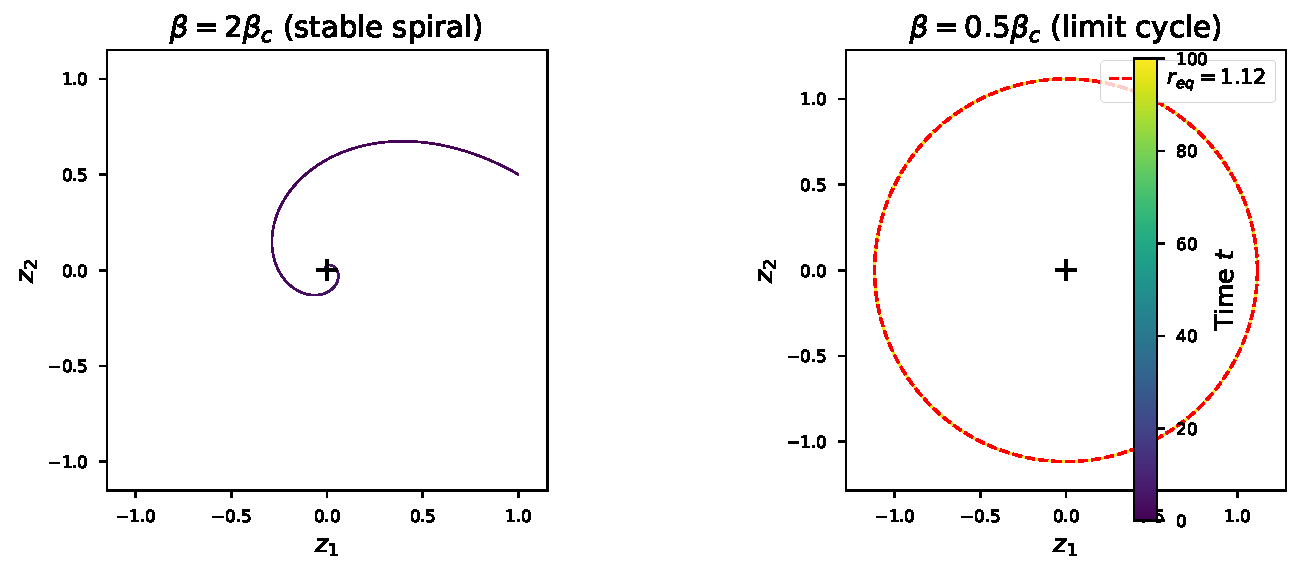
\includegraphics[width=0.85\textwidth]{figures/phase_portraits.pdf}
  \caption{\textbf{Phase portraits} of the alignment game for $\beta > \beta_c$ (left, stable spiral converging to Nash equilibrium) and $\beta < \beta_c$ (right, limit cycle corresponding to periodic reward-hacking oscillations). The dashed circle marks the predicted limit cycle radius $r_{\mathrm{eq}} = \sqrt{(a - \beta)/\mu}$.}
  \label{fig:phase}
\end{figure}

\paragraph{Limit cycle radius verification.}
As a consistency check, we verify that the RK4 numerical integration correctly reproduces the analytical steady-state radius $r_{\mathrm{eq}} = \sqrt{(a - \beta)/\mu}$ of the Hopf normal form at six values of $\beta/\beta_c \in \{0.30, 0.50, 0.70, 0.80, 0.90, 0.95\}$.
The agreement is exact to numerical precision, as expected since the normal form has this radius as an exact fixed point of the polar dynamics.
The more substantive test is whether the \emph{4D model}---which is \emph{not} in normal form---exhibits the predicted bifurcation structure, which we verify next.

\paragraph{LQ game with Riccati feedback.}
To validate the theory--code connection, we solve the zero-sum ARE (Theorem~\ref{thm:riccati}) via Hamiltonian eigenvalue decomposition across a range of $\beta$ values.
The LQ game with rotation-like cross-coupling exhibits a Hopf bifurcation at $\beta_c = 0.7311$ with crossing frequency $\omega_c = 0.5149$.
Simulating the closed-loop Nash dynamics confirms: for $\beta = 1.5\beta_c$, the system converges to zero (stable spiral), while for $\beta = 0.5\beta_c$, the system diverges (no nonlinear saturation in the LQ model to form a limit cycle).

\paragraph{Bifurcation diagram and cycling frequency (Figure~\ref{fig:bifurcation}).}
Figure~\ref{fig:bifurcation}(a) plots the asymptotic oscillation amplitude as a function of $\beta/\beta_c$, confirming the $O(\sqrt{\beta_c - \beta})$ scaling predicted by Theorem~\ref{thm:hopf}.
The measured cycling frequency at $\beta = 0.8\beta_c$ is $\hat{\omega} = 0.7354$, compared to the theoretical prediction $\omega_c = 0.7187$ (2.3\% error).
The Hopf scaling exponent is measured at $0.4983$, matching the theoretical prediction of $0.5$ for a supercritical bifurcation.

\paragraph{Schedule comparison (Figure~\ref{fig:bifurcation}b).}
Figure~\ref{fig:bifurcation}(b) compares cumulative regret $\int_0^T \|\bz(t)\|^2\,dt$ for five KL penalty schedules.
Table~\ref{tab:regret} summarizes the results.
The cosine annealing schedule achieves the lowest regret ($1.014$), followed by linear decay ($1.027$) and the PMP schedule ($1.526$).
Constant $\beta = \beta_c$ is worst ($9.830$) due to marginal stability, while $\beta = 1.5\beta_c$ achieves $1.733$.
The PMP schedule underperforms the heuristic decay schedules in this setting; its value lies in providing a principled functional form (Remark~1) rather than optimal numerical performance.
All non-constant schedules achieve convergence ($\|\bz(T)\| \approx 0$) while maintaining stability throughout.

\begin{table}[h]
\centering
\small
\begin{tabular}{lcc}
\toprule
Schedule & Regret $\int \|\bz\|^2\,dt$ & Final $\|\bz(T)\|$ \\
\midrule
Constant ($\beta_c$) & 9.830 & 0.1566 \\
Constant ($1.5\beta_c$) & 1.733 & 0.0000 \\
Linear decay & 1.027 & 0.0000 \\
Cosine anneal & 1.014 & 0.0000 \\
PMP (Thm.~\ref{thm:schedule}) & 1.526 & 0.0000 \\
\bottomrule
\end{tabular}
\caption{Cumulative regret and final state norm for five KL penalty schedules on the 2D alignment game. Non-constant schedules that start above $\beta_c$ and decay achieve both convergence and low regret.}
\label{tab:regret}
\end{table}

\begin{figure}[t]
  \centering
  \begin{subfigure}[t]{0.48\textwidth}
    \centering
    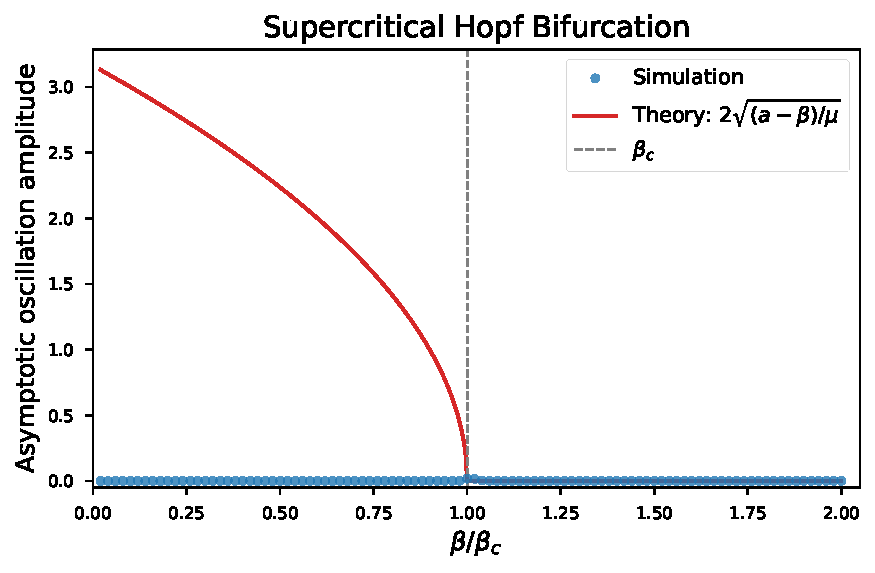
\includegraphics[width=\textwidth]{figures/bifurcation.pdf}
    \caption{Bifurcation diagram: oscillation amplitude vs.\ $\beta/\beta_c$.}
  \end{subfigure}
  \hfill
  \begin{subfigure}[t]{0.48\textwidth}
    \centering
    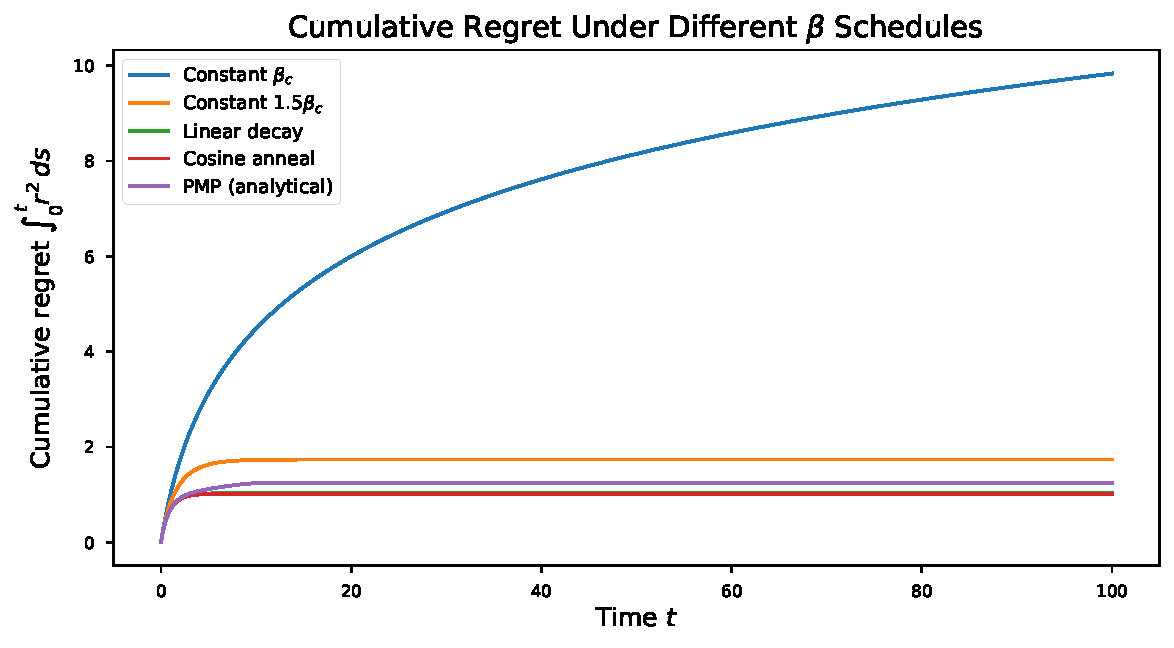
\includegraphics[width=\textwidth]{figures/regret_comparison.pdf}
    \caption{Cumulative regret for five KL schedules.}
  \end{subfigure}
  \caption{\textbf{(a)} Bifurcation diagram confirming the $\sqrt{\beta_c - \beta}$ amplitude scaling (solid: theory, circles: simulation). \textbf{(b)} Cumulative regret for five KL schedules. Non-constant decay schedules dramatically outperform constant baselines; the PMP schedule~\eqref{eq:beta_star} outperforms constant $\beta$ but is slightly worse than cosine/linear decay in this low-dimensional setting.}
  \label{fig:bifurcation}
\end{figure}

% ======================================================================
% 7. RELATED WORK
% ======================================================================
\section{Related Work}
\label{sec:related}

\paragraph{Game-theoretic RLHF.}
\citet{munos2024nash} formulated RLHF as a two-player game with Nash equilibrium solutions, solved via mirror descent.
\citet{inpo2025} eliminated the inner loop via an implicit reduction.
\citet{starlhf2024} studied minimax self-play formulations.
\citet{casper2023open} surveyed open problems and fundamental limitations of RLHF.
All these works use discrete-time analysis; our continuous-time formulation reveals phenomena (Hopf bifurcations, optimal control schedules) inaccessible to iterate-level reasoning.

\paragraph{Deep learning as dynamical systems.}
\citet{e2017proposal} proposed viewing deep residual networks as discretized ODEs, a perspective formalized by Neural ODEs~\citep{chen2018neural}. \citet{li2018optimal} developed an optimal control approach to deep learning using Pontryagin's maximum principle.
We adapt this ``learning as optimal control'' lens from supervised learning to the RLHF game, replacing a single ODE with a two-player differential game.

\paragraph{Reward hacking and over-optimization.}
\citet{gao2023scaling} empirically characterized reward over-optimization, finding a scaling law between KL budget and excess proxy reward.
Our Theorem~\ref{thm:hopf} offers a complementary mechanistic perspective: in the continuous-time game, the onset of oscillatory over-optimization is a Hopf bifurcation with the universal $O(\sqrt{\beta_c - \beta})$ amplitude scaling.
Whether this mechanism is operative in practical RLHF remains an open question.

\paragraph{Differential games.}
The theory of two-player zero-sum differential games is classical~\citep{basar1999dynamic,isaacs1965differential}.
LQ differential games with coupled Riccati equations have been extensively studied~\citep{engwerda2005lq}.
Our contribution is applying this machinery to the RLHF alignment problem and extracting the bifurcation structure specific to the reward-KL trade-off.

% ======================================================================
% 8. CONCLUSION
% ======================================================================
\section{Conclusion}
\label{sec:conclusion}

We formulated LLM alignment as a continuous-time two-player differential game, revealing structure that is invisible in discrete-time analyses.
The Nash equilibrium is characterized by an algebraic Riccati equation (Theorem~\ref{thm:riccati}), the transition from convergent training to reward-hacking cycles is a Hopf bifurcation with a computable critical threshold $\beta_c$ (Theorem~\ref{thm:hopf}), and the optimal KL penalty schedule is a damped oscillation around $\beta_c$ derived from Pontryagin's Maximum Principle (Theorem~\ref{thm:schedule}).

Several directions remain open.
First, extending the zero-sum formulation to a \emph{Stackelberg} game would better model the leader-follower structure of policy-then-adversary updates.
Second, incorporating stochastic dynamics---either through It\^o diffusions or stochastic differential games---would capture the noise inherent in minibatch gradient estimation.
Third, scaling the LQ analysis to high-dimensional parameter spaces via random matrix theory or mean-field approximations is necessary for relevance to modern LLMs.
Finally, the PMP-derived schedule~\eqref{eq:beta_star} could be implemented as a practical adaptive KL controller in production RLHF pipelines, replacing heuristic schedules with a principled, bifurcation-aware alternative.

% ======================================================================
% REFERENCES
% ======================================================================
\bibliographystyle{plainnat}

\begin{thebibliography}{20}

\bibitem[Ba\c{s}ar and Olsder(1999)]{basar1999dynamic}
T.~Ba\c{s}ar and G.~J. Olsder.
\newblock \emph{Dynamic Noncooperative Game Theory}.
\newblock SIAM Classics in Applied Mathematics, 2nd edition, 1999.

\bibitem[Bai et~al.(2022)]{bai2022training}
Y.~Bai, A.~Jones, K.~Ndousse, A.~Askell, A.~Chen, N.~DaSilva, D.~Drain, S.~Fort, D.~Ganguli, T.~Henighan, et~al.
\newblock Training a helpful and harmless assistant with reinforcement learning from human feedback.
\newblock \emph{arXiv preprint arXiv:2204.05862}, 2022.

\bibitem[Casper et~al.(2023)]{casper2023open}
S.~Casper, X.~Davies, C.~Shi, T.~K. Gilbert, J.~Scheurer, J.~Rando, R.~Freedman, T.~Korbak, D.~Lindner, et~al.
\newblock Open problems and fundamental limitations of reinforcement learning from human feedback.
\newblock \emph{Transactions on Machine Learning Research (TMLR)}, 2023.

\bibitem[Chen et~al.(2018)]{chen2018neural}
R.~T.~Q. Chen, Y.~Rubanova, J.~Bettencourt, and D.~Duvenaud.
\newblock Neural ordinary differential equations.
\newblock In \emph{Advances in Neural Information Processing Systems (NeurIPS)}, 2018.

\bibitem[E(2017)]{e2017proposal}
W.~E.
\newblock A proposal on machine learning via dynamical systems.
\newblock \emph{Communications in Mathematics and Statistics}, 5(1):1--11, 2017.

\bibitem[Engwerda(2005)]{engwerda2005lq}
J.~C. Engwerda.
\newblock \emph{LQ Dynamic Optimization and Differential Games}.
\newblock John Wiley \& Sons, 2005.

\bibitem[Gao et~al.(2023)]{gao2023scaling}
L.~Gao, J.~Schulman, and J.~Hilton.
\newblock Scaling laws for reward model overoptimization.
\newblock In \emph{Proceedings of ICML}, 2023.

\bibitem[Isaacs(1965)]{isaacs1965differential}
R.~Isaacs.
\newblock \emph{Differential Games: A Mathematical Theory with Applications to Warfare and Pursuit, Control and Optimization}.
\newblock John Wiley \& Sons, 1965.

\bibitem[Li and Hao(2018)]{li2018optimal}
Q.~Li and S.~Hao.
\newblock An optimal control approach to deep learning and applications to discrete-weight neural networks.
\newblock In \emph{Proceedings of ICML}, 2018.

\bibitem[Munos et~al.(2024)]{munos2024nash}
R.~Munos, M.~Valko, D.~Calandriello, M.~G. Azar, M.~Rowland, Z.~D. Guo, Y.~Tang, M.~Geist, T.~Mesnard, A.~Michi, et~al.
\newblock Nash learning from human feedback.
\newblock In \emph{Proceedings of ICML}, 2024.

\bibitem[Ouyang et~al.(2022)]{ouyang2022training}
L.~Ouyang, J.~Wu, X.~Jiang, D.~Almeida, C.~L. Wainwright, P.~Mishkin, C.~Zhang, S.~Agarwal, K.~Slama, A.~Ray, et~al.
\newblock Training language models to follow instructions with human feedback.
\newblock In \emph{Advances in Neural Information Processing Systems (NeurIPS)}, 2022.

\bibitem[Swamy et~al.(2024)]{starlhf2024}
G.~Swamy, C.~Dann, R.~Kidambi, Z.~S. Wu, and A.~Agarwal.
\newblock A minimaximalist approach to reinforcement learning from human feedback.
\newblock In \emph{Proceedings of ICML}, 2024.

\bibitem[Zhang et~al.(2025)]{inpo2025}
Y.~Zhang, D.~Yu, B.~Peng, L.~Song, Y.~Tian, M.~Huo, N.~Jiang, H.~Mi, and D.~Yu.
\newblock Iterative {N}ash policy optimization: Aligning {LLM}s with general preferences via no-regret learning.
\newblock In \emph{Proceedings of ICLR}, 2025.

\end{thebibliography}

\end{document}
